% ECHO: paper source. Plain article class on purpose; the venue template
% (IEEEtran for ICDE, acmart for WWW/SIGIR) is swapped in at the end and
% only this preamble changes. Every \cite key exists in references.bib and
% was verified against the paper's own page (see related_work.md).
\documentclass[10pt,twocolumn]{article}
\usepackage[margin=0.75in]{geometry}
% shared preamble (packages, colours, macros); input by main.tex and build.sh
\usepackage[T1]{fontenc}
\usepackage[utf8]{inputenc}
\usepackage{lmodern}
\usepackage{amsmath,amssymb,amsthm}
\usepackage{booktabs,multirow,array}
\usepackage{graphicx}
\usepackage{xcolor}
\usepackage{tikz}
\usetikzlibrary{arrows.meta,positioning,calc,shapes.misc,backgrounds,fit}
\usepackage{pgfplots}
\pgfplotsset{compat=1.17}
\usepackage[hidelinks]{hyperref}
\usepackage[nameinlink,capitalize]{cleveref}
\usepackage{microtype}
% float placement: let wide figures sit at the top or bottom of the page
% they are referenced on, and do not let one deferred figure* hold back
% every later float
\usepackage{dblfloatfix}
\renewcommand{\topfraction}{0.95}
\renewcommand{\bottomfraction}{0.95}
\renewcommand{\textfraction}{0.05}
\renewcommand{\floatpagefraction}{0.8}
\renewcommand{\dbltopfraction}{0.95}
\renewcommand{\dblfloatpagefraction}{0.8}
\setcounter{topnumber}{3}
\setcounter{dbltopnumber}{3}
\setcounter{totalnumber}{5}

\usepackage{caption}
\captionsetup{font=small,labelfont=bf}

\newtheorem{proposition}{Proposition}
\newtheorem{definition}{Definition}

% colours shared by every figure
\definecolor{cDyad}{HTML}{2A6F97}
\definecolor{cPath}{HTML}{E07A1F}
\definecolor{cStruct}{HTML}{4C9A2A}
\definecolor{cPop}{HTML}{8E6BBF}
\definecolor{cComp}{HTML}{C0392B}
\definecolor{cGrey}{HTML}{6B6B6B}
\definecolor{cLight}{HTML}{F2F4F7}


% Figures: use the pre-rendered PDF when it exists (fast on Overleaf's free
% plan), otherwise draw the TikZ source. build_figs.sh makes the PDFs.
\newcommand{\figfile}[2]{%
  \IfFileExists{figures/#1.pdf}{\includegraphics[width=#2]{figures/#1.pdf}}{\input{figures/#1}}}

\newcommand{\model}{ECHO}
\newcommand{\hone}{H@1}
\newcommand{\hten}{H@10}
\newcommand{\dyad}[2]{(#1,#2)}
\newcommand{\lam}{\lambda}
\newcommand{\spm}{\ensuremath{\,\scriptstyle\pm\,}}



\title{\model{}: Dyadic Event-Stream Intensities for\\Temporal Knowledge Graph Forecasting}

\author{%
  Authors to be added\\
  Computer Network Information Center, Chinese Academy of Sciences\\
  University of Chinese Academy of Sciences\\
  Beijing, China
}
\date{}

\begin{document}
\maketitle

\begin{abstract}
Temporal knowledge graph forecasting asks which object completes a query $(s, r, ?, t)$ given every fact before $t$. The strongest published models answer it by reading the history of the query pair $(s, r)$: a copy mechanism over its past objects, or a graph built from its past facts. We show that this is the wrong unit of evidence. The unit that carries the signal is the \emph{dyad}, the ordered entity pair $(s, o)$ together with the typed, timestamped stream of every event between them under any relation and in either direction. On ICEWS18, 23\% of test queries have an answer that never occurred with $(s, r)$ yet had interacted with $s$ before; every copy mechanism is silent on them by construction. A counter that merely reads the dyad, with no trained parameter, already matches DaeMon on that benchmark.

We present \model{}, which treats a query as a draw from a superposition of four marked point processes whose intensities are added, never gated: a structural intensity from snapshot evolution, a popularity intensity over all entities, a dyadic intensity in which a small Transformer encodes the dyad's event stream, and a path intensity that forwards each dyadic state along the candidate's own most recent typed edges. Candidates of one query attend to one another before they are scored, so an intensity can depend on what the competing candidates' streams look like.

Over three seeds and five benchmarks, \model{} sets the best published MRR and \hone{} on YAGO (91.82 / 90.57) and WIKI (83.41 / 80.44), the best \hone{} on GDELT (18.16), and on ICEWS18 and ICEWS14s exceeds every model whose code we could run under one protocol. A stratified evaluation, defined from the data alone, shows where each intensity acts: the dyadic stream and its relation types matter on event data and not on yearly data, exactly where the dyad stratum exists. Code, result files and the diagnostic are released.
\end{abstract}

\section{Introduction}
\label{sec:intro}

A temporal knowledge graph (TKG) records facts as quadruples $(s, r, o, t)$: a subject $s$ and an object $o$ linked by relation $r$ at time $t$. Forecasting on a TKG means completing $(s, r, ?, t)$ from the facts strictly before $t$. The benchmarks are political event streams (ICEWS, GDELT) and yearly encyclopaedic graphs (YAGO, WIKI), and the task has drawn a dense line of work over six years: recurrent graph encoders~\cite{jin2020renet,li2021regcn,li2022cen,dong2025dimnet}, copy mechanisms~\cite{zhu2021cygnet,xu2023cenet}, path and rule reasoners~\cite{han2021xerte,sun2021titer,liu2022tlogic,dong2023daemon,dong2024tipnn,gastinger2026counttrucola}, global history graphs~\cite{li2022tirgn,chen2024logcl,zhang2024hisres,chen2025cogntke} and, most recently, diffusion models~\cite{cai2024diffutkg,nadex2026,freqdiff2026}.

A recurring finding runs through this literature and is easy to underrate. A baseline that only looks up which objects recurred for $(s, r)$ in the past, with a handful of hand-set parameters, is competitive with or better than most published models on three of five benchmarks~\cite{gastinger2024history}. A counter with no temporal information at all reaches \hten{} above 0.9 on some of them~\cite{zhang2026evolution}. Over 80\% of ICEWS test events have happened before~\cite{strikingness2026}. Progress, in other words, is measured on a task whose majority is repetition, and the methods that win have in common that they read the history of the query pair $(s, r)$ very well.

\begin{figure}[!tb]
  \centering
  \figfile{fig_intro}{\linewidth}
  \caption{\textbf{What \model{} reads.} Countries linked by dated, typed events, and the question: whom will the United States consult on March 14? A copy mechanism reads only the thin \emph{consult} arrows, so Russia is not a candidate for it. \model{} reads every event between the United States and each country as one ordered stream; for Russia that stream, an agreement, a criticism and a statement within weeks, says the two are in close contact, and \model{} ranks Russia first. On ICEWS18 the answer is visible only in this reading for 23.4\% of test queries (\cref{sec:diag}). Names and dates are illustrative.}
  \label{fig:intro}
\end{figure}

\paragraph{The unit of evidence.} This paper starts from a question the copy family cannot ask. For a query $(s, r, ?, t)$, what if every past event between $s$ and a candidate $o$ were allowed to speak, under any relation and in either direction, with its type and its time? We call the ordered pair $(s, o)$ with that stream a \emph{dyad} (\cref{fig:intro}). The question has an answer that is a property of the data, not of any model (\cref{sec:diag}). On ICEWS18 the test queries split into three disjoint strata: 50.6\% whose answer already occurred with $(s, r)$, 23.4\% whose answer never did but had interacted with $s$ under some other relation, and 26.0\% whose answer never interacted with $s$ at all. The second stratum is invisible to a copy mechanism by construction. A hand-built counter that reads the dyad instead of the triple, with the same time decay and no training, lifts the untrained score on ICEWS18 from MRR 28.0 to 31.8, which is the level of DaeMon~\cite{dong2023daemon}, and on ICEWS14 from 37.1 to 43.3, which is the level of TLogic~\cite{liu2022tlogic}.

\paragraph{The model.} \model{} is built on that measurement. A query is a draw from a superposition of marked point processes, and the intensities add (\cref{sec:method}). The dyadic intensity encodes the last $L$ events of the dyad as a sequence of (relation, elapsed time) tokens with a two-layer Transformer, so that recurrence, cross-relation excitation, reciprocity and order all enter through one mechanism and nothing is confined to decay monotonically in time. Because a dyad is only instantiated when it has history, the per-pair point process that earlier work dismissed as combinatorially infeasible~\cite{han2020ghnn} costs a few dozen sequences per query. Two further intensities extend the reach of the dyad: a path intensity forwards each dyadic state along the candidate's own most recent typed edges, reaching the 54\% of ``cold'' answers that are partners of a partner, and a popularity intensity scores every entity from multi-scale decayed counts. A structural intensity from snapshot evolution, which is prior work~\cite{li2021regcn,dong2025dimnet}, completes the superposition. Finally, the candidates of one query attend to one another before they are scored, so the intensity of a candidate can depend on what the other candidates' streams look like.

\paragraph{What we claim, and what we do not.} Over three seeds and five benchmarks (\cref{sec:exp}), \model{} reports the best published MRR and \hone{} on YAGO and WIKI, the best \hone{} on GDELT, and on ICEWS18 and ICEWS14s it is above every model whose code we could run under a single protocol, including LogCL~\cite{chen2024logcl}, which we re-ran. Three recent methods report higher ICEWS numbers~\cite{zhang2024hisres,lei2026cidtkg,lei2026chetkg}; none has released code, and evaluation settings in this field are known to move results by several points~\cite{gastinger2023apples}. We therefore state the comparison exactly as it is rather than pool numbers across protocols. The contribution we stand on is not a leaderboard margin but a mechanism and a measurement: the dyad stratum exists, it is large on event data and empty on yearly data, and the stratified evaluation in \cref{sec:analysis} shows the dyadic stream and its relation types act precisely where that stratum is (ICEWS18: $+0.58$ and $+0.43$ MRR) and not where it is not (YAGO: $0.00$ and $-0.03$).

\paragraph{Contributions.}
\begin{itemize}\setlength\itemsep{0pt}
  \item A data-only diagnostic that partitions test queries into recurrent, dyad-only and cold strata, and the measurement that the dyad-only stratum is a quarter of ICEWS queries and that an untrained dyad counter matches DaeMon.
  \item \model{}, a superposition of four intensities built around a Transformer over the dyad's typed event stream, with a path intensity that composes a dyadic state with a typed edge and a competition layer across the candidates of a query.
  \item Three-seed results on five benchmarks, ablations on an event and a yearly dataset, and a stratified analysis that attributes each intensity to the stratum it was built for. All code, the diagnostic and every result file are released.
\end{itemize}

\section{Related Work}
\label{sec:related}

\paragraph{Recurrence and copy mechanisms.}
CyGNet~\cite{zhu2021cygnet} introduced a copy mode that scores the objects that already answered the same $(s, r)$ in the past, next to a generation mode over the whole vocabulary, on the observation that many facts recur. CENET~\cite{xu2023cenet} learns whether a query follows its historical or its non-historical dependency and applies the decision as a mask at inference. TiRGN~\cite{li2022tirgn} pairs a local recurrent graph encoder with a global history encoder for repeated facts and a time-guided decoder with periodicity. Gastinger et al.~\cite{gastinger2024history} showed that a non-learned recurrency baseline is competitive with eleven published models on three of five benchmarks, and CountTRuCoLa~\cite{gastinger2026counttrucola} turned that observation into four rule types with confidence functions that combine recency and frequency. All of these define ``history'' as the past of the query pair $(s, r)$. The dyad-only stratum of \cref{sec:diag}, where the answer interacted with $s$ under another relation, lies outside that definition by construction.

\paragraph{Snapshot evolution.}
RE-NET~\cite{jin2020renet} and RE-GCN~\cite{li2021regcn} evolve entity representations through a sequence of snapshot graphs, with a relational GCN per snapshot and a recurrent unit across them; CEN~\cite{li2022cen} adds a length-aware CNN with curriculum learning and an online setting; DiMNet~\cite{dong2025dimnet} adds cross-time links at equal hop depth and a disentanglement of active and stable node features. HiSMatch~\cite{li2022hismatch} frames the task as matching the query's historical structure against each candidate's. Our structural intensity is this family and is claimed as nothing more than the backbone; trained alone it reaches RE-GCN's level on ICEWS18 (\cref{sec:analysis}).

\paragraph{Global history graphs.}
The strongest recent results come from models that build a query-specific graph from the whole history and run message passing over it. LogCL~\cite{chen2024logcl} samples the one-hop facts of the query subject and the one-hop facts of the objects that answered $(s, r)$ before, applies entity-aware attention, and regularises the fusion of local and global views with four contrast patterns. HisRES~\cite{zhang2024hisres} aggregates all historical facts of the query pair into a global relevance graph and merges it with a multi-granularity recent encoder; its own ablation attributes six MRR points on ICEWS18 to that graph. CID-TKG and CHE-TKG~\cite{lei2026cidtkg,lei2026chetkg} add a second graph of recent facts retrieved through temporal logical rules and align the two views contrastively. CognTKE~\cite{chen2025cogntke} runs a fast one-hop and a slow multi-hop reasoner over a relation digraph. \model{} reads the same facts as event streams rather than as a graph: the stream encoder sees the order and the types of a dyad's events, the path intensity composes a stream with a typed edge, and nothing is contextualised by a second GNN. Of the three strongest members of this family, none has released code; the comparison in \cref{sec:exp} says so explicitly.

\paragraph{Paths, rules and explanation.}
xERTE~\cite{han2021xerte} expands a query-centred subgraph with temporal attention; TITer~\cite{sun2021titer} walks it with a reinforcement-learning agent; DaeMon~\cite{dong2023daemon} carries a path memory between the query subject and every candidate without entity representations, and TiPNN~\cite{dong2024tipnn} reasons over query-aware temporal paths on a unified history graph. TLogic~\cite{liu2022tlogic} extracts temporal logical rules by temporal random walks. Our untrained typed-dyad counter behaves like TLogic's length-one rules and reaches its ICEWS14 score; the path intensity is a learned form of its length-two rules, with the rule body read from an event stream instead of a single past fact.

\paragraph{Point processes.}
Know-Evolve~\cite{trivedi2017knowevolve} modelled each fact as a multivariate point process whose intensity is a function of evolving entity embeddings. GHNN~\cite{han2020ghnn} extended the neural Hawkes process to graph sequences and argued that treating every possible link as its own event-type dimension is infeasible because the number of types explodes. GAttNHP~\cite{tian2026gattnhp} encodes subject--relation chains as continuous-time point processes with grouped Hawkes priors. \model{} keeps the point-process reading and resolves the combinatorial objection: a dyad is instantiated only when it has history, so the per-pair process costs a few dozen short sequences per query, and its kernel is a learned function of a sinusoidal time encoding rather than a decay.

\paragraph{Diffusion models.}
DiffuTKG~\cite{cai2024diffutkg} casts the prediction as denoising the target fact with a Transformer conditioned on the query's history; NADEx~\cite{nadex2026} adds batch-wise negative prototypes to the conditioning and FreqDiff~\cite{freqdiff2026} a spectral calibration. These are orthogonal to the evidence question we study and are included in the comparison with their own reported numbers.

\paragraph{Evaluation.}
Gastinger et al.~\cite{gastinger2023apples} documented that filter settings, prediction horizon and dataset versions move TKG forecasting results by several points and distort comparisons; the recurrency baseline~\cite{gastinger2024history}, the co-occurrence shortcut of Zhang et al.~\cite{zhang2026evolution}, strikingness-aware reweighting~\cite{strikingness2026} and the synthetic shift benchmark of \"Ozdemir et al.~\cite{shift2026} all say that aggregate metrics on these benchmarks are dominated by repetition. The stratified evaluation of \cref{sec:analysis} is the real-data counterpart of probing mechanisms separately, and it is why we re-ran the one strong competitor with code under our protocol instead of quoting it.

\paragraph{Different settings.}
Inductive reasoning over emerging entities~\cite{transfir2026,adatkg2026} and continual fine-tuning at test time~\cite{hitscl2026} report gains under their own protocols. Our cold strata are not the emerging-entity problem: both entities are known, they have simply never interacted.

\section{Preliminaries}
\label{sec:prelim}

\paragraph{Task.}
A temporal knowledge graph is a set of quadruples $\mathcal{G} = \{(s, r, o, t)\}$ over entities $\mathcal{E}$ ($|\mathcal{E}| = N$), relations $\mathcal{R}$ and discrete timestamps $t \in \{0, \dots, T-1\}$. We re-index time to the rank of the timestamp on the full timeline, so that one step is one snapshot on every dataset whatever the raw unit (a day on ICEWS, fifteen minutes on GDELT, a year on YAGO and WIKI). Following every method we compare with, each fact is augmented with its inverse $(o, r^{-1}, s, t)$, giving $2|\mathcal{R}|$ relation types, and a query is $(s, r, ?, t)$ with $r$ ranging over both directions. The model ranks all $N$ entities as the object using only facts with timestamp strictly less than $t$; at test time the true history before $t$ is available, which is the setting of RE-GCN and its successors~\cite{li2021regcn}.

\paragraph{Protocol.}
We report MRR and Hits@$k$ under the time-aware filter: for a query $(s, r, ?, t)$, the other true objects of $(s, r)$ \emph{at time $t$} are removed from the ranking and nothing else is. Ties are resolved to their average rank, $1 + \#\{\text{better}\} + (\#\{\text{tied}\} - 1)/2$. The optimistic rule that counts only strictly better scores credits a model with rank~1 whenever thousands of entities share the target's score, which a copy-style model produces by default; we found it inflates \hten{} on YAGO to 99.9 against a published ceiling of 93.3, and we do not use it. Model selection is on validation MRR; test is evaluated once with the selected checkpoint.

\paragraph{Dyads and strata.}
For a query $(s, r, ?, t)$ and a candidate $o$, the \emph{dyad stream} $\mathcal{D}_{so}(t)$ is the time-ordered sequence of all events $(\rho, \tau)$ with $\tau < t$ such that $(s, \rho, o, \tau) \in \mathcal{G}$, where $\rho$ ranges over both directions, so an event in which $o$ acted on $s$ appears with the inverse type. The \emph{triple history} is the sub-stream with $\rho = r$. These two sets induce a partition of the test queries that is defined from the data alone:

\begin{definition}[Strata]
\label{def:strata}
A test query with answer $o^\star$ is \textbf{recurrent} if $(s, r, o^\star, \tau) \in \mathcal{G}$ for some $\tau < t$; \textbf{dyad-only} if it is not recurrent but $\mathcal{D}_{so^\star}(t)$ is non-empty; and \textbf{cold} otherwise. A recurrent query is further \textbf{blocked} if some $o' \neq o^\star$ with triple history is both at least as recent and at least as frequent as $o^\star$, and \textbf{clean} otherwise. A cold query is \textbf{cold-2hop} if $o^\star$ is a partner of one of the $P_1$ most recent partners of $s$, and \textbf{cold-far} otherwise.
\end{definition}

The blocked stratum is the set no scorer of the form $f(\text{count}) \cdot g(\Delta t)$ with $f$ non-decreasing and $g$ non-increasing can order correctly, whatever its parameters: the dominating distractor scores at least as high on both arguments. Every copy mechanism we know of is of that form. The dyad-only stratum is the set where such a scorer has no input at all.

\section{What the Dyad Knows: A Data-Only Diagnostic}
\label{sec:diag}

Before any model is trained we ask two questions of the data. How large are the strata of \cref{def:strata}? And does reading the dyad instead of the triple carry ranking information? Both are answered with hand-built counters that share one time decay $w(\Delta) = e^{-0.3\Delta} + 0.2\,e^{-0.02\Delta} + 0.02$ (in snapshots) and read only events before the query time. No parameter is fitted to the test set; the one learned quantity, a relation-to-relation confidence, is counted on the training split.

\begin{itemize}\setlength\itemsep{1pt}
  \item \textbf{Recurrence} scores $o$ by $\sum w(\Delta)$ over past $(s, r, o)$ events. This is the copy family and the strict recurrency baseline of \cite{gastinger2024history}.
  \item \textbf{Blind dyad} scores $o$ by $\sum w(\Delta)$ over every past event between $s$ and $o$, relation ignored.
  \item \textbf{Typed dyad} weights each of those events by $\mathrm{conf}(\rho \to r)$, the training-split frequency with which a $\rho$-event on a dyad is followed by an $r$-event within seven steps. This is a length-one temporal rule in the sense of TLogic~\cite{liu2022tlogic}.
  \item \textbf{Popularity} scores $o$ by $\sum w(\Delta)$ over all past $(\cdot, r, o)$ events, the relaxed recurrency of \cite{gastinger2024history}.
  \item \textbf{Backoff} orders by recurrence, then the typed dyad, then popularity.
\end{itemize}

\begin{figure}[t]
  \centering
  \figfile{fig_strata}{\linewidth}
  \caption{\textbf{Strata are a property of the data.} Share of test queries whose answer is recurrent (occurred with $(s, r)$ before), dyad-only (never with $(s, r)$, but $s$ and the answer interacted under another relation or direction) and cold (never interacted). A copy mechanism is silent on the dyad-only stratum by construction. It is a quarter of the ICEWS queries and absent from YAGO and WIKI.}
  \label{fig:strata}
\end{figure}

\Cref{fig:strata} gives the first answer. On both ICEWS benchmarks about half of the test queries are recurrent, a quarter are dyad-only and a quarter are cold. On YAGO and WIKI the dyad-only stratum is 0.1\%: facts there persist for years and the pair's history is the triple's history. The diagnostic therefore makes a prediction before any model exists: a mechanism that reads the dyad should help on ICEWS and should not help on YAGO or WIKI. \Cref{sec:analysis} tests it.

\begin{table}[t]
  \centering\small
  \caption{\textbf{Untrained counters.} Time-aware filtered, ties averaged, $\times 100$. ICEWS18 on a random sample of 30\,000 test queries, ICEWS14s on all. The only learned quantity is a relation-to-relation confidence counted on the training split. Published DaeMon on ICEWS18: 31.85 / 22.67 / 49.80~\cite{dong2025dimnet}; TLogic on ICEWS14: 43.04 / 33.56 / 61.23~\cite{liu2022tlogic}.}
  \label{tab:diag}
  \begin{tabular}{llrrr}
    \toprule
    dataset & counter & MRR & \hone{} & \hten{} \\
    \midrule
    \multirow{5}{*}{ICEWS18}
      & recurrence  & 28.02 & 20.93 & 41.41 \\
      & blind dyad  & 24.55 & 14.71 & 45.10 \\
      & typed dyad  & 30.65 & 21.05 & 49.82 \\
      & popularity  & 12.09 &  6.64 & 23.13 \\
      & backoff     & \textbf{31.82} & \textbf{22.55} & \textbf{49.88} \\
    \midrule
    \multirow{5}{*}{ICEWS14s}
      & recurrence  & 37.08 & 30.80 & 48.50 \\
      & blind dyad  & 36.78 & 26.43 & 57.31 \\
      & typed dyad  & 42.72 & 33.73 & 60.39 \\
      & popularity  & 15.50 &  8.21 & 30.19 \\
      & backoff     & \textbf{43.26} & \textbf{34.08} & \textbf{60.85} \\
    \bottomrule
  \end{tabular}
\end{table}

\Cref{tab:diag} gives the second answer. Allowing the whole dyad to speak lifts the untrained score on ICEWS18 from MRR 28.0 to 31.8 and \hten{} from 41.4 to 49.9, and on ICEWS14s from 37.1 to 43.3. The ICEWS18 figure is the published level of DaeMon and the ICEWS14s figure that of TLogic, neither of which is a weak model. On the dyad-only stratum alone, where recurrence scores exactly zero, the blind dyad counter reaches \hone{} 9.5 and \hten{} 42.3 on ICEWS18 and \hten{} 61.8 on ICEWS14s.

Two things the counters do \emph{not} show are worth stating, because the model is designed around them. First, on the dyad-only stratum the typed counter is no better than the blind one (ICEWS18 MRR 20.33 against 20.01): the gain of the dyad comes from reading the pair at all, and whether relation types carry more than an additive confidence can extract is left to a learned sequence model. Second, the cold stratum is reached by none of the counters. A further measurement (\texttt{diagnose\_paths.py}) shows that 54\% of cold answers on ICEWS18 are partners of one of the subject's 96 most recent partners, inside a set of about 555 entities, which is 2.4\% of the vocabulary; a hand-built two-hop path counter combined with popularity reaches MRR 4.5 on that stratum against 2.9 for popularity alone. The path intensity of \cref{sec:method} is built for those queries.

\section{\model{}}
\label{sec:method}

\begin{figure*}[t]
  \centering
  % Architecture overview. Four coloured lanes (structural, popularity,
% dyadic, path) feeding one logaddexp. Pure TikZ, no external images.
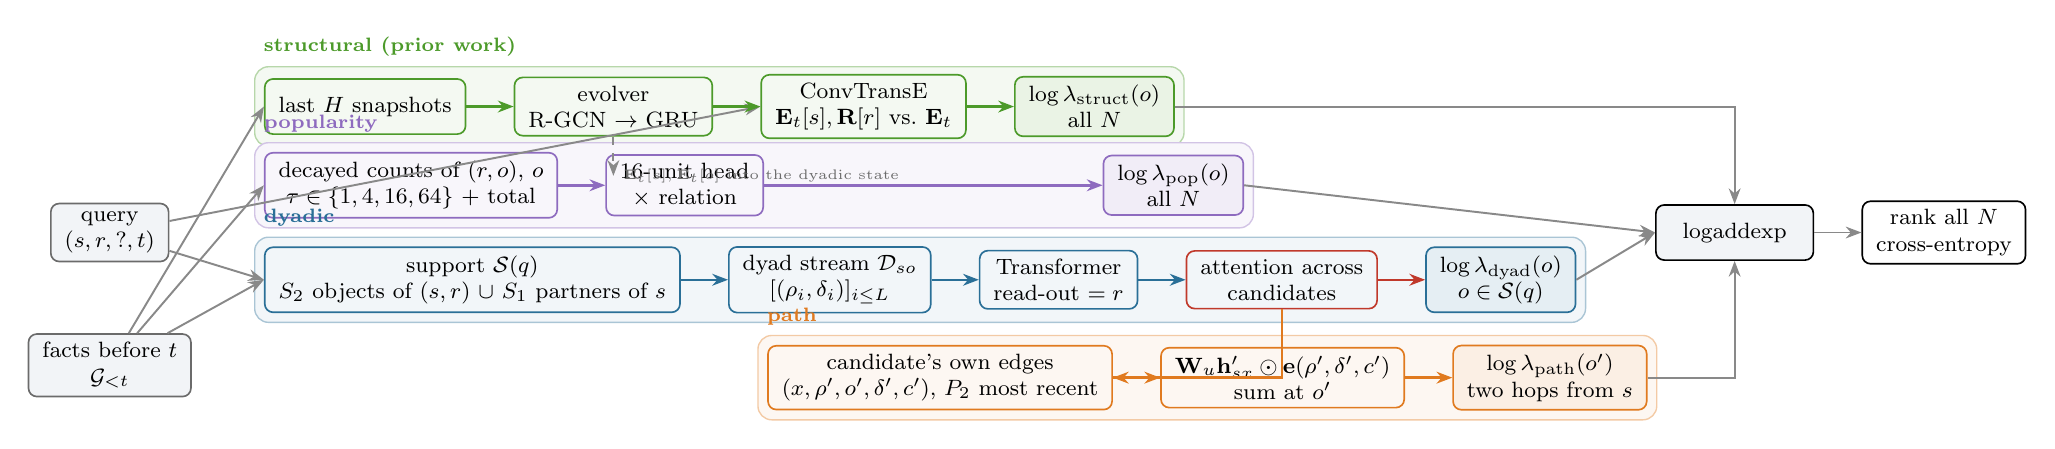
\begin{tikzpicture}[
  font=\footnotesize,
  box/.style={draw, rounded corners=3pt, minimum height=7mm, inner xsep=5pt, inner ysep=3pt, align=center, line width=0.6pt},
  lane/.style={rounded corners=5pt, fill=#1!6, draw=#1!40, line width=0.5pt},
  arr/.style={-{Stealth[length=2mm]}, line width=0.7pt, cGrey!80},
  carr/.style={-{Stealth[length=2mm]}, line width=0.9pt, #1},
  lab/.style={font=\scriptsize\bfseries, text=#1},
  node distance=4mm and 6mm,
]
% ── query ─────────────────────────────────────────────────────────────────
\node[box, fill=cLight, draw=cGrey] (q) {query\\$(s, r, ?, t)$};
\node[box, fill=cLight, draw=cGrey, below=9mm of q] (hist) {facts before $t$\\$\mathcal{G}_{<t}$};

% ── structural lane ───────────────────────────────────────────────────────
\node[box, draw=cStruct, right=12mm of q, yshift=16mm] (snap) {last $H$ snapshots};
\node[box, draw=cStruct, right=of snap] (evo) {evolver\\R-GCN $\to$ GRU};
\node[box, draw=cStruct, right=of evo] (conv) {ConvTransE\\$\mathbf{E}_t[s], \mathbf{R}[r]$ vs.\ $\mathbf{E}_t$};
\node[box, draw=cStruct, fill=cStruct!12, right=of conv] (ls) {$\log\lambda_{\text{struct}}(o)$\\all $N$};

% ── popularity lane ───────────────────────────────────────────────────────
\node[box, draw=cPop, right=12mm of q, yshift=6mm] (cnt) {decayed counts of $(r,o)$, $o$\\$\tau \in \{1,4,16,64\}$ + total};
\node[box, draw=cPop, right=of cnt] (poph) {16-unit head\\$\times$ relation};
\node[box, draw=cPop, fill=cPop!12, right=of poph, xshift=37mm] (lp) {$\log\lambda_{\text{pop}}(o)$\\all $N$};

% ── dyadic lane ───────────────────────────────────────────────────────────
\node[box, draw=cDyad, right=12mm of q, yshift=-6mm] (sup) {support $\mathcal{S}(q)$\\$S_2$ objects of $(s,r)$ $\cup$ $S_1$ partners of $s$};
\node[box, draw=cDyad, right=of sup] (str) {dyad stream $\mathcal{D}_{so}$\\$[(\rho_i,\delta_i)]_{i\le L}$};
\node[box, draw=cDyad, right=of str] (tr) {Transformer\\read-out $= r$};
\node[box, draw=cComp, right=of tr] (comp) {attention across\\candidates};
\node[box, draw=cDyad, fill=cDyad!12, right=of comp] (ld) {$\log\lambda_{\text{dyad}}(o)$\\$o \in \mathcal{S}(q)$};

% ── path lane ─────────────────────────────────────────────────────────────
\node[box, draw=cPath, below=of str, xshift=14mm] (edge) {candidate's own edges\\$(x,\rho',o',\delta',c')$, $P_2$ most recent};
\node[box, draw=cPath, right=of edge] (msg) {$\mathbf{W}_u \mathbf{h}'_{sx} \odot \mathbf{e}(\rho',\delta',c')$\\sum at $o'$};
\node[box, draw=cPath, fill=cPath!12, right=of msg] (lpath) {$\log\lambda_{\text{path}}(o')$\\two hops from $s$};

% ── combination ───────────────────────────────────────────────────────────
\node[box, draw=black, fill=cLight, right=10mm of ld, yshift=6mm, minimum width=20mm] (lae) {$\operatorname{logaddexp}$};
\node[box, draw=black, right=of lae] (out) {rank all $N$\\cross-entropy};

% ── lanes background ──────────────────────────────────────────────────────
\begin{scope}[on background layer]
  \node[lane=cStruct, fit=(snap)(ls)] (L1) {};
  \node[lane=cPop,    fit=(cnt)(lp)]  (L2) {};
  \node[lane=cDyad,   fit=(sup)(ld)]  (L3) {};
  \node[lane=cPath,   fit=(edge)(lpath)] (L4) {};
\end{scope}
\node[lab=cStruct, anchor=south west] at (L1.north west) {structural (prior work)};
\node[lab=cPop, anchor=south west] at (L2.north west) {popularity};
\node[lab=cDyad, anchor=south west] at (L3.north west) {dyadic};
\node[lab=cPath, anchor=south west] at (L4.north west) {path};

% ── arrows ────────────────────────────────────────────────────────────────
\draw[arr] (hist) -- (snap.west);
\draw[arr] (hist) -- (cnt.west);
\draw[arr] (hist) -- (sup.west);
\draw[arr] (q) -- (sup.west);
\draw[arr] (q) -- (conv.west);
\draw[carr=cStruct] (snap) -- (evo); \draw[carr=cStruct] (evo) -- (conv); \draw[carr=cStruct] (conv) -- (ls);
\draw[carr=cPop] (cnt) -- (poph); \draw[carr=cPop] (poph) -- (lp);
\draw[carr=cDyad] (sup) -- (str); \draw[carr=cDyad] (str) -- (tr); \draw[carr=cDyad] (tr) -- (comp); \draw[carr=cComp] (comp) -- (ld);
\draw[carr=cPath] (comp.south) |- (edge.east) ;
\draw[carr=cPath] (edge) -- (msg); \draw[carr=cPath] (msg) -- (lpath);
\draw[arr] (ls.east) -| (lae.north);
\draw[arr] (lp.east) -- (lae.west);
\draw[arr] (ld.east) -- (lae.west);
\draw[arr] (lpath.east) -| (lae.south);
\draw[arr] (lae) -- (out);
\draw[arr, dashed] (evo.south) -- ++(0,-5mm) node[right, font=\tiny, text=cGrey] {$\mathbf{E}_t[s], \mathbf{E}_t[o]$ into the dyadic state};
\end{tikzpicture}

  \caption{\textbf{Overview of \model{}.} A query $(s, r, ?, t)$ is scored by four intensities that are added as intensities, never gated. The \textcolor{cStruct}{structural} intensity evolves entity states through the last $H$ snapshots and decodes against every entity. The \textcolor{cPop}{popularity} intensity scores every entity from multi-scale decayed counts of $(r, o)$ and of $o$. The \textcolor{cDyad}{dyadic} intensity builds the support of $s$, encodes each candidate's typed event stream with a Transformer whose read-out token is the query relation, lets the candidates of the query \textcolor{cComp}{attend to one another}, and scores each one. The \textcolor{cPath}{path} intensity forwards every candidate's state along that candidate's own most recent typed edges and sums the messages arriving at each second-hop entity. The four log-intensities are combined by $\mathrm{logaddexp}$ and trained with one cross-entropy over all $N$ entities.}
  \label{fig:overview}
\end{figure*}

\subsection{A superposition of intensities}

We model the object of a query $q = (s, r, ?, t)$ as the mark of the first event of a superposition of marked point processes. Superposition adds intensities, so if $\lam_k(o \mid q)$ is the intensity under which $o$ would be emitted by process $k$, the probability that the answer is $o$ is proportional to $\sum_k \lam_k(o \mid q)$, and in log space the branches combine through
\begin{equation}
  \begin{aligned}
  \log \lam(o \mid q) = \operatorname{logaddexp}\big(&\log\lam_{\text{struct}}(o \mid q),\ \log\lam_{\text{pop}}(o \mid q),\\
                                                      &\log\lam_{\text{dyad}}(o \mid q),\ \log\lam_{\text{path}}(o \mid q)\big).
  \end{aligned}
  \label{eq:super}
\end{equation}
There is no mixing weight and no gate. A learned gate between a copy branch and a neural branch is the usual design in this literature, and in our own earlier attempts it either collapsed onto one branch or oscillated between epochs; a sum of intensities has neither failure mode, and a branch that is uninformative for a query simply contributes a small intensity. Each branch has its own learned bias, initialised at $-2$, so that all four start at comparable scale. The model is trained with cross-entropy over all $N$ entities on $\operatorname{softmax}_o \log\lam(o \mid q)$, with label smoothing, plus a small auxiliary cross-entropy on the structural branch alone that keeps it from being starved by the easier branches during the first epochs.

\subsection{Support}

The dyadic and path intensities act on a \emph{support} $\mathcal{S}(q) \subset \mathcal{E}$ built from the subject's past alone: the $S_2$ objects that most recently occurred with $(s, r)$ and the $S_1$ entities with which $s$ most recently interacted under any relation, in either direction, de-duplicated. With $S_1 = 96$ and $S_2 = 64$ the support covers every recurrent and dyad-only answer of ICEWS18 except those of hub subjects with more partners than the budget. Everything the two intensities read about a candidate is computed from events strictly before $t$ by vectorised prefix operations over the subject's event list, once per timestamp and shared by all queries at that timestamp; \cref{sec:exp} reports the cost.

\subsection{Dyadic intensity}

For each candidate $o \in \mathcal{S}(q)$ the last $L$ events of the dyad stream $\mathcal{D}_{so}(t)$, most recent first, become tokens
\begin{equation}
  \mathbf{x}_i = \mathbf{E}_\rho[\rho_i] + \phi(\delta_i), \qquad i = 1, \dots, L,
\end{equation}
where $\rho_i \in \{1, \dots, 2|\mathcal{R}|\}$ is the typed, directed relation of the $i$-th event and $\delta_i = t - \tau_i \ge 1$ its elapsed time in snapshots. The time encoding is
\begin{equation}
  \begin{aligned}
  \phi(\delta) &= \mathbf{W}_\phi \big[\tfrac{1}{4}\ell,\ \sin(\omega_1 \ell), \cos(\omega_1 \ell),\\
               &\qquad\quad \dots,\ \sin(\omega_8 \ell), \cos(\omega_8 \ell)\big], \qquad \ell = \log(1 + \delta),
  \end{aligned}
  \label{eq:time}
\end{equation}
with $\omega_k$ geometrically spaced in $[1, 24]$. Nothing in \cref{eq:time} is monotone in $\delta$, so the intensity built on it can peak at any elapsed time the data asks for, which a decay kernel cannot. A read-out token $\mathbf{q} = \mathbf{E}_q[r] + \mathbf{W}_s \mathbf{E}_t[s]$ carries the query relation and the evolved subject state; the sequence $[\mathbf{q}; \mathbf{x}_1; \dots; \mathbf{x}_L]$ passes through two pre-norm Transformer blocks with four heads and dimension 64, and the output at the read-out position is the stream state $\mathbf{z}_{so}$. One mechanism therefore covers self-excitation (past $r$ events on the dyad, which is recurrence), cross-excitation (past $\rho \ne r$ events raising $r$), reciprocity (events in the other direction, which carry the inverse type) and order (the sequence $\rho_1 \rho_2$ differs from $\rho_2 \rho_1$).

Truncating the stream to $L$ events must not lose counts, so the state is concatenated with eight summary statistics of the full history, $\mathbf{a}_{so} = [\log(1+n_{sro}), \log(1+\delta_{sro}), \log(1+\bar{g}_{sro}), \mathbf{1}[n_{sro} > 0], \log(1+n_{so}), \log(1+\delta_{so}), \log(1+\bar{g}_{so}), n_{sro}/n_{so}]$, where $n$, $\delta$ and $\bar{g}$ are the count, the recency and the mean inter-arrival gap of the triple $(s, r, o)$ and of the dyad $(s, o)$. The candidate is also described by what \emph{it} has been doing with anyone: its $P_2$ most recent distinct typed edges $(\rho', o', \delta', c')$, each embedded as $\mathbf{E}_{\rho'} + \phi(\delta') + \mathbf{W}_c \log(1 + c')$, are mean-pooled into a context vector $\mathbf{c}_o$. The per-candidate state is then
\begin{equation}
  \mathbf{h}_{so} = \mathrm{MLP}\big([\mathbf{z}_{so};\ \mathrm{LN}(\mathbf{a}_{so});\ \mathbf{W}_e \mathbf{E}_t[o];\ \mathbf{c}_o;\ \mathbf{q}_s;\ \mathbf{q}_r]\big),
\end{equation}
with $\mathbf{q}_s = \mathbf{W}_s' \mathbf{E}_t[s]$ and $\mathbf{q}_r = \mathbf{W}_r \mathbf{R}[r]$.

\paragraph{Competition.}
A scorer that looks at one candidate at a time cannot express ``the answer rotates among these partners'' or ``the partner that has gone quiet is due''. The states of all candidates of one query therefore pass through one further attention block \emph{across the support}, masked to the valid candidates, so that $\mathbf{h}'_{so}$ depends on the streams of the other candidates. The dyadic log-intensity is a linear read-out, $\log\lam_{\text{dyad}}(o \mid q) = \mathbf{w}^\top \mathbf{h}'_{so} + b_{\text{dyad}}$, and is $-\infty$ outside the support. On the yearly datasets, where a query rarely has more than one candidate with a live triple history, the competition block is switched off; \cref{sec:exp} states how that choice was made.

\subsection{Path intensity}

The dyad is silent whenever $s$ and the answer never interacted, which is a quarter of the ICEWS queries. The path intensity extends the reach of the dyad by one hop. Each first-hop candidate $x \in \mathcal{S}(q)$ forwards its query-conditioned state along its own $P_2$ most recent typed edges $(x, \rho', o', \delta', c')$:
\begin{equation}
  \begin{aligned}
  \mathbf{m}_{x \to o'} &= (\mathbf{W}_u \mathbf{h}'_{sx}) \odot \mathbf{e}(\rho', \delta', c'),\\
  \mathbf{e}(\rho', \delta', c') &= \mathrm{MLP}\big(\mathbf{E}'_{\rho'} + \phi(\delta') + \mathbf{W}_c' \log(1+c')\big),
  \end{aligned}
\end{equation}
and the messages arriving at each second-hop entity $o'$ are summed, $\bar{\mathbf{m}}_{o'} = n_{o'}^{-1/2} \sum_x \mathbf{m}_{x \to o'}$ over the $n_{o'}$ paths that reach it, excluding paths back to $s$. The path log-intensity is
\begin{equation}
  \begin{aligned}
  \log\lam_{\text{path}}(o' \mid q) = \mathrm{MLP}\big([&\mathrm{LN}(\bar{\mathbf{m}}_{o'});\ \log(1+n_{o'});\\
                                                        &\mathbf{W}_e \mathbf{E}_t[o'];\ \mathbf{q}_s;\ \mathbf{q}_r]\big) + b_{\text{path}},
  \end{aligned}
\end{equation}
and $-\infty$ for entities no path reaches. A path is thus the composition of a full event stream, read by the Transformer, with a typed, timed edge: a differentiable length-two temporal rule whose body is a sequence rather than a single past fact. Because every first-hop state is already computed, the path costs one sparse gather and one scatter-add per chunk of queries.

\subsection{Popularity and structural intensities}

The popularity intensity scores \emph{every} entity from evidence rather than from an embedding alone. For a timestamp $t$ and the relations present in its queries, decayed counts of $(\cdot, r, o)$ events at scales $\tau \in \{1, 4, 16, 64\}$ snapshots and an undecayed total, and the same five counts of $o$ under any relation, are computed on the device by one scatter over the events before $t$. The ten log-counts pass through a 16-unit layer modulated by the relation embedding and a linear read-out, giving $\log\lam_{\text{pop}}(o \mid q)$ for all $o$. This is the relaxed-recurrency signal of \cite{gastinger2024history} in learned, multi-scale form, without a top-$k$ cut.

The structural intensity is the backbone of this literature and is not a contribution. Entity states $\mathbf{E}_t$ are obtained by evolving the static table $\mathbf{E}_0$ through the $H$ snapshots before $t$ with a relational message-passing layer that keeps mean and max aggregates and links each layer to the same depth at the previous snapshot, a GRU cell across snapshots, and a gate back to $\mathbf{E}_0$; a ConvTransE decoder with LayerNorm scores $\mathbf{E}_t[s]$ and $\mathbf{R}[r]$ against all of $\mathbf{E}_t$. LayerNorm replaces the customary BatchNorm because batches are snapshots of very uneven size that are further chunked, and batch statistics would make the objective depend on the chunking. Trained alone this branch reaches the published level of RE-GCN (\cref{sec:analysis}).

\subsection{Training}

Training iterates over timestamps. For a timestamp $t$ the structural states and the popularity table are computed once, the graph is cut there, and the queries at $t$ are processed in chunks bounded by a budget on (query, candidate) pairs; each chunk's loss is backpropagated to the detached states, whose accumulated gradients are then carried once through the evolver and the popularity head. The gradient is identical to that of a single backward pass and memory is bounded by one chunk. Supports, streams and second-hop edges are built by vectorised prefix operations over the subject's and the candidates' event lists, in data-loader workers, with nothing later than $t-1$ ever read; a released script deletes every event at or after $t$ and checks bit-for-bit that nothing the model reads at $t$ changes.

\section{Experiments}
\label{sec:exp}

\subsection{Setup}

\paragraph{Datasets.}
We use the five standard benchmarks in the versions released with RE-GCN and CEN~\cite{li2021regcn,li2022cen}: ICEWS14s (7\,128 entities, 230 relations, 365 daily snapshots), ICEWS18 (23\,033 / 256 / 304), GDELT (7\,691 / 240 / 2\,975 fifteen-minute snapshots), YAGO (10\,623 / 10 / 189 yearly) and WIKI (12\,554 / 24 / 232 yearly), with the usual chronological 80/10/10 split. No auxiliary data is used: in particular, we do not use the static entity-type graph that RE-GCN and its descendants optionally add on ICEWS.

\paragraph{Baselines.}
The comparison in \cref{tab:main} quotes each number from the paper that produced it and names the source, because numbers produced by different harnesses are not interchangeable~\cite{gastinger2023apples}. Rows for CyGNet, xERTE, TITer, RE-GCN, CEN, DaeMon, TiPNN and DiMNet on ICEWS18 and GDELT come from the DiMNet table~\cite{dong2025dimnet}; rows on YAGO and WIKI from the DaeMon table~\cite{dong2023daemon}; LogCL, HisRES, CID-TKG and CHE-TKG from their own papers; the diffusion rows from NADEx and FreqDiff; CognTKE, the recurrency baseline and CountTRuCoLa from their own papers. We additionally re-ran LogCL, the strongest competitor with released code, under our protocol on ICEWS18; it reaches MRR 36.0 there, consistent with its published 35.67. Methods marked $\dagger$ have not released code at the time of writing and could not be re-run.

\paragraph{Implementation.}
Entity and relation dimension 200, two message-passing layers, history $H = 10$ snapshots ($5$ on GDELT), stream length $L = 10$ ($16$ on YAGO and WIKI, $8$ on GDELT), stream dimension 64 with two blocks of four heads, support $S_1 = 96$, $S_2 = 64$ ($48$ on YAGO and WIKI), second-hop edges $P_2 = 16$, path dimension 32. AdamW with learning rate $10^{-3}$, weight decay $10^{-3}$, 5\% linear warm-up then cosine to $2 \cdot 10^{-5}$, at most 20 epochs with early stopping after 6 epochs without validation improvement, gradient clipping at 1, label smoothing 0.1 (0.05 on YAGO and WIKI), dropout 0.25 on event data and 0.15 on yearly data, structural auxiliary weight 0.3 (0 on YAGO and WIKI). The competition block is on for the event datasets and off for YAGO and WIKI; validation MRR makes that choice on all five datasets (for it: ICEWS18 36.92 vs 36.70, ICEWS14s 48.99 vs 48.81, GDELT 27.45 vs 27.38; against it: YAGO 87.41 vs 87.14, WIKI 83.38 vs 83.29), and both test results are reported in \cref{tab:compete}. Training runs in bfloat16 on one A100-40GB; an ICEWS18 epoch takes about 3 minutes and a run about 50 minutes, GDELT about 15 minutes per epoch. Every number is the mean of three seeds (1, 2, 3) with its standard deviation.

\subsection{Main results}

\begin{table*}[t]
  \centering\small
  \caption{\textbf{Main results}, time-aware filtered, $\times 100$. Each baseline number is quoted from the paper named in the source column; \model{} is the mean of three seeds (standard deviations in \cref{tab:compete}). $\dagger$: no released code. Best in \textbf{bold}, second \underline{underlined}. ICEWS14s rows other than DiMNet, LogCL, NADEx and \model{} are from the CID-TKG table.}
  \label{tab:main}
  \setlength{\tabcolsep}{3pt}
  \resizebox{\textwidth}{!}{%
  \begin{tabular}{l l rrr rrr rrr rrr rrr}
    \toprule
    & & \multicolumn{3}{c}{ICEWS18} & \multicolumn{3}{c}{ICEWS14s} & \multicolumn{3}{c}{GDELT} & \multicolumn{3}{c}{YAGO} & \multicolumn{3}{c}{WIKI} \\
    \cmidrule(lr){3-5}\cmidrule(lr){6-8}\cmidrule(lr){9-11}\cmidrule(lr){12-14}\cmidrule(lr){15-17}
    method & source & MRR & \hone{} & \hten{} & MRR & \hone{} & \hten{} & MRR & \hone{} & \hten{} & MRR & \hone{} & \hten{} & MRR & \hone{} & \hten{} \\
    \midrule
    Recurrency baseline & \cite{gastinger2024history} & 28.7 & -- & -- & -- & -- & -- & 24.5 & -- & -- & 90.9 & -- & -- & 81.5 & -- & -- \\
    CyGNet   & \cite{dong2025dimnet,dong2023daemon} & 24.93 & 15.90 & 42.61 & -- & -- & -- & 18.48 & 11.52 & 31.98 & 52.07 & 45.36 & 63.77 & 33.89 & 29.06 & 41.86 \\
    xERTE    & \cite{dong2025dimnet,dong2023daemon} & 29.31 & 21.03 & 45.60 & -- & -- & -- & 18.09 & 12.30 & 30.34 & 84.19 & 80.09 & 89.78 & 71.14 & 68.05 & 79.01 \\
    TITer    & \cite{dong2025dimnet,dong2023daemon} & 29.98 & 22.05 & 44.83 & -- & -- & -- & 15.46 & 10.98 & 24.31 & 87.47 & 84.89 & 90.27 & 75.50 & 72.96 & 79.02 \\
    RE-GCN   & \cite{dong2025dimnet,dong2023daemon,lei2026cidtkg} & 30.58 & 21.01 & 48.75 & 42.39 & 31.96 & 62.29 & 19.64 & 12.42 & 33.69 & 84.12 & 80.76 & 89.98 & 77.55 & 73.75 & 83.68 \\
    CEN      & \cite{dong2025dimnet} & 30.84 & 21.23 & 49.67 & -- & -- & -- & 20.18 & 12.84 & 34.10 & -- & -- & -- & -- & -- & -- \\
    TiRGN    & \cite{lei2026cidtkg} & 33.66 & 23.19 & 54.22 & 44.75 & 34.26 & 65.28 & 21.67 & 13.63 & 37.60 & -- & -- & -- & -- & -- & -- \\
    DaeMon   & \cite{dong2025dimnet,dong2023daemon} & 31.85 & 22.67 & 49.80 & -- & -- & -- & 20.73 & 13.65 & 34.23 & \underline{91.59} & \underline{90.03} & \textbf{93.34} & 82.38 & 78.26 & \textbf{88.01} \\
    TiPNN    & \cite{dong2025dimnet} & 32.17 & 22.74 & 50.72 & -- & -- & -- & 21.17 & 14.03 & 34.76 & -- & -- & -- & -- & -- & -- \\
    CountTRuCoLa & \cite{gastinger2026counttrucola} & 32.8 & -- & -- & -- & -- & -- & 23.8 & -- & -- & 90.9 & -- & -- & 82.7 & -- & -- \\
    DiMNet   & \cite{dong2025dimnet} & 34.13 & 23.29 & 55.80 & 45.72 & 34.41 & 67.99 & 21.93 & 14.03 & 37.49 & -- & -- & -- & -- & -- & -- \\
    CognTKE  & \cite{chen2025cogntke} & 35.24 & -- & -- & -- & -- & -- & -- & -- & -- & -- & -- & -- & \underline{83.21} & -- & -- \\
    LogCL    & \cite{chen2024logcl} & 35.67 & 24.53 & 57.74 & 48.87 & 37.76 & 70.26 & 23.75 & 14.64 & 42.33 & -- & -- & -- & -- & -- & -- \\
    DiffuTKG & \cite{freqdiff2026} & 35.65 & 25.19 & 59.55 & 47.58 & 36.38 & 66.01 & 21.35 & 14.43 & 36.05 & -- & -- & -- & -- & -- & -- \\
    NADEx    & \cite{nadex2026} & 36.84 & 27.58 & 60.58 & 49.03 & 39.45 & 70.55 & 23.67 & 16.10 & 43.05 & -- & -- & -- & -- & -- & -- \\
    FreqDiff$^\dagger$ & \cite{freqdiff2026} & 36.85 & 26.85 & \underline{61.47} & 50.85 & 39.82 & 71.48 & 25.04 & 17.64 & 41.83 & -- & -- & -- & -- & -- & -- \\
    HisRES$^\dagger$   & \cite{zhang2024hisres} & 37.69 & 26.46 & 59.70 & 50.48 & 39.57 & 71.09 & 26.58 & 16.90 & \underline{46.31} & -- & -- & -- & -- & -- & -- \\
    CHE-TKG$^\dagger$  & \cite{lei2026chetkg} & \underline{38.77} & \underline{27.58} & 60.95 & \underline{51.91} & \underline{41.37} & \underline{72.17} & \underline{27.38} & \underline{17.73} & 47.02 & -- & -- & -- & -- & -- & -- \\
    CID-TKG$^\dagger$  & \cite{lei2026cidtkg} & \textbf{38.88} & \textbf{27.66} & 61.16 & \textbf{51.93} & \textbf{41.49} & \textbf{72.32} & \textbf{27.41} & \underline{17.76} & \textbf{47.03} & -- & -- & -- & -- & -- & -- \\
    \midrule
    \model{} (ours) & & 36.54 & 26.36 & 56.21 & 47.43 & 37.49 & 66.16 & 27.10 & \textbf{18.16} & 44.62 & \textbf{91.82} & \textbf{90.57} & \underline{93.23} & \textbf{83.41} & \textbf{80.44} & \underline{87.39} \\
    \bottomrule
  \end{tabular}}
\end{table*}

\Cref{tab:main} reports the comparison. We read it in three parts and state each exactly.

\textbf{YAGO and WIKI.} \model{} is above every published number we found on MRR and \hone{} on both yearly benchmarks, including DaeMon, which held them for three years, and CognTKE's WIKI MRR. On \hten{} DaeMon remains ahead by 0.1 and 0.6 points. The three-seed spread is 0.20 MRR on YAGO and 0.12 on WIKI, so the \hone{} margins of 0.54 and 2.18 are well outside it.

\textbf{GDELT.} \model{} has the best \hone{} of any published method, 18.16 against 17.76 for CID-TKG, and the second MRR, 0.3 behind CID-TKG and above HisRES and every method with code. The seed spread is 0.02.

\textbf{ICEWS18 and ICEWS14s.} \model{} is above every method with released code, including LogCL both as published and as re-run under our protocol, DiMNet, NADEx and the diffusion models on ICEWS18 MRR. It is below HisRES, CHE-TKG and CID-TKG, which report 1.2 to 2.3 more MRR on ICEWS18 and 3 to 4.5 more on ICEWS14s, and none of which has released code. We do not claim those gaps are protocol artefacts; we note only that gaps of this size are within what differences in evaluation settings have been shown to produce in this field~\cite{gastinger2023apples}, and that the one member of the family we could re-run reproduced its published number. The \hten{} gap to this family (4 to 6 points) is larger than the MRR gap and is where \model{} is weakest; \cref{sec:analysis} locates it in the cold strata.

\begin{table}[t]
  \centering\small
  \caption{\textbf{Competition across candidates}, test MRR / \hone{}, three seeds. Validation MRR selects the setting in bold on every dataset; the unselected setting is reported for completeness.}
  \label{tab:compete}
  \begin{tabular}{lcc}
    \toprule
    dataset & without competition & with competition \\
    \midrule
    ICEWS18  & 36.29 \spm0.04 / 26.10 & \textbf{36.54 \spm0.10 / 26.36} \\
    ICEWS14s & 47.18 \spm0.04 / 37.19 & \textbf{47.43 \spm0.14 / 37.49} \\
    GDELT    & 27.01 \spm0.01 / 18.05 & \textbf{27.10 \spm0.02 / 18.16} \\
    WIKI     & \textbf{83.41 \spm0.12 / 80.44} & 83.28 \spm0.17 / 80.22 \\
    YAGO     & \textbf{91.82 \spm0.20 / 90.57} & 91.62 \spm0.12 / 90.33 \\
    \bottomrule
  \end{tabular}
\end{table}

\paragraph{Competition.}
\Cref{tab:compete} isolates the one per-dataset switch. Attention across the candidates of a query adds 0.25 MRR on ICEWS18, 0.25 on ICEWS14s and 0.09 on GDELT, in the same direction on every seed, and removes 0.13 and 0.20 on WIKI and YAGO. The diagnostic predicts this: on the yearly datasets a query rarely has more than one candidate with a live triple history, so there is nothing to compete, and the extra block only adds variance. Validation MRR makes the same choice as test on all five datasets, which is why the switch is a dataset setting rather than a tuned result.

\paragraph{Training behaviour.}
Every run selects its checkpoint between epochs 5 and 12 of 20, and the structural branch alone needs 17. A model that reads the history directly has little to memorise. Ten alternative recipes on ICEWS18 (16- and 20-epoch schedules, dropout 0.35 and 0.45, weight decay $10^{-3}$, learning rate $5 \cdot 10^{-4}$, auxiliary weight 0 and 1, label smoothing 0.2, wider supports) all land between 36.0 and 36.3 MRR and all peak at epochs 8 to 10; the plateau is a property of what the model can see, not of regularisation, and the ablations of \cref{sec:analysis} say which parts of what it sees matter.

\section{Analysis}
\label{sec:analysis}

The aggregate numbers of \cref{tab:main} say how much; this section says where and why. Every stratum is defined from the data alone (\cref{def:strata}) and partitions the test set, so the rows of each table weight to the aggregate.

\subsection{Where the queries are, and where the errors are}

\begin{table}[t]
  \centering\small
  \caption{\textbf{Performance by stratum} on ICEWS18 and ICEWS14s (three seeds, model without competition so that the rows match the ablation base; the competition setting moves the aggregates by 0.25). Strata partition the test set.}
  \label{tab:strata}
  \setlength{\tabcolsep}{2.8pt}\footnotesize
  \begin{tabular}{l rrrr rrrr}
    \toprule
    & \multicolumn{4}{c}{ICEWS18} & \multicolumn{4}{c}{ICEWS14s} \\
    \cmidrule(lr){2-5}\cmidrule(lr){6-9}
    stratum & share & MRR & \hone{} & \hten{} & share & MRR & \hone{} & \hten{} \\
    \midrule
    cold-far   & 17.8\% &  1.84 &  0.64 &  3.18 & 15.9\% &  2.01 &  0.41 &  4.12 \\
    cold-2hop  & 14.0\% &  8.93 &  3.13 & 19.46 & 12.0\% & 11.57 &  3.54 & 28.64 \\
    dyad-only  & 19.2\% & 29.71 & 17.21 & 56.72 & 21.2\% & 37.26 & 23.45 & 66.82 \\
    blocked    & 25.7\% & 34.99 & 16.82 & 72.96 & 16.6\% & 38.43 & 17.64 & 79.93 \\
    clean      & 23.4\% & 85.64 & 76.65 & 99.02 & 34.4\% & 89.93 & 83.32 & 99.34 \\
    \bottomrule
  \end{tabular}
\end{table}

\Cref{tab:strata} is the central table of the paper. On ICEWS18 the clean stratum, where the answer recurred for $(s, r)$ and dominates every distractor on recency and count, is a quarter of the queries and is essentially solved (\hten{} 99.0). The blocked stratum, the same size, is where a monotone copy score provably cannot order the answer first; \model{} ranks it first 16.8\% of the time and in the top ten 73\% of the time, so the ordering information it uses is not count-and-recency. The dyad-only stratum, a fifth of the queries and invisible to every copy mechanism, reaches MRR 29.7 and \hten{} 56.7: the untrained blind-dyad counter reached 20.0 and 42.3 on the same stratum (\cref{sec:diag}), and the learned stream adds ten points on top of it. The two cold strata, a third of the queries, are where the model is weak: an answer that is a partner of a partner is found in the top ten one time in five, and an answer that is further than two hops from the subject is almost never found. The \hten{} gap to the global-graph family in \cref{tab:main} is of the order of the mass in these two rows, and we take it to be where the next step lies.

\subsection{Ablations}

\begin{table}[t]
  \centering\small
  \caption{\textbf{Ablations} on an event dataset and a yearly dataset: MRR and its change relative to the model without competition. Rows marked $^{3}$ are three-seed means (spread at most 0.19); the others are seed 1. The seed spread of the base is 0.04 on ICEWS18 and 0.20 on YAGO. \hone{} moves with MRR in every row (ICEWS18 base 26.10, without the dyadic branch 20.51; YAGO base 90.57, without it 61.37).}
  \label{tab:ablation}
  \setlength{\tabcolsep}{4pt}\footnotesize
  \begin{tabular}{l rr rr}
    \toprule
    & \multicolumn{2}{c}{ICEWS18} & \multicolumn{2}{c}{YAGO} \\
    \cmidrule(lr){2-3}\cmidrule(lr){4-5}
    removed & MRR & $\Delta$ & MRR & $\Delta$ \\
    \midrule
    nothing (base)$^{3}$           & 36.29 &         & 91.82 & \\
    popularity field               & 36.37 & $+0.08$ & 91.81 & $-0.01$ \\
    candidate context              & 36.27 & $-0.02$ & 91.75$^{3}$ & $-0.07$ \\
    path intensity                 & 35.92 & $-0.37$ & 91.70$^{3}$ & $-0.12$ \\
    relation types in the stream   & 35.86 & $-0.43$ & 91.79 & $-0.03$ \\
    the stream (statistics only)   & 35.71 & $-0.58$ & 91.83 & $+0.01$ \\
    structural branch              & 35.59 & $-0.70$ & 90.97 & $-0.85$ \\
    dyadic branch                  & 30.30 & $-5.99$ & 67.18 & $-24.64$ \\
    \midrule
    \emph{added} competition$^{3}$ & 36.54 & $+0.25$ & 91.62 & $-0.20$ \\
    \bottomrule
  \end{tabular}
\end{table}

\Cref{tab:ablation} removes one part at a time on ICEWS18, where the dyad-only stratum is 19\% of the queries, and on YAGO, where it is 0.1\%. Three readings follow.

\textbf{The dyadic branch is the model.} Without it \model{} is a snapshot encoder with a popularity prior and scores 30.30 on ICEWS18, which is RE-GCN's published 30.58, and 67.18 on YAGO. The branch is worth 6.0 MRR on the event dataset and 24.6 on the yearly one.

\textbf{The stream acts where the diagnostic said it would.} On ICEWS18 the Transformer over the event stream is worth 0.58 MRR over the eight summary statistics alone, and the relation types inside it are worth 0.43: a stream with types replaced by a single placeholder loses most of what the stream adds. The path intensity adds 0.37, and \cref{tab:strata} locates it: on cold-2hop queries it lifts MRR from 6.21 to 8.52 and \hten{} from 13.4 to 19.0 on seed 1. The seed spread on ICEWS18 is 0.04, so each of these effects is an order of magnitude above noise. On YAGO the same three parts are worth $+0.01$, $-0.03$ and $-0.12$, all inside the 0.20 seed spread. The eight statistics carry the dyadic branch on their own there, because on yearly data the question is only whether a fact is still running, and the count and recency of the triple answer it. This is the prediction made in \cref{sec:diag} before any model was trained, and it is the kind of evidence a stratum-level analysis can give and a leaderboard cannot.

\textbf{Two parts are null and are reported as such.} The popularity field and the candidate-context input move neither dataset outside the seed spread; a prototype intensity that scores every entity by similarity to the query's past answers, tried for the cold-far stratum, is likewise null ($+0.05$ on ICEWS18, $-0.16 \pm 0.19$ on YAGO) and is kept only as an ablation switch. We leave them in the released code with their switches rather than silently removing them, so that the ablation table is reproducible as printed.

\subsection{The same strata on every event dataset}

\begin{figure}[t]
  \centering
  % MRR of the final model by stratum on the three event datasets
% (three seeds, model without competition; from collect.py).
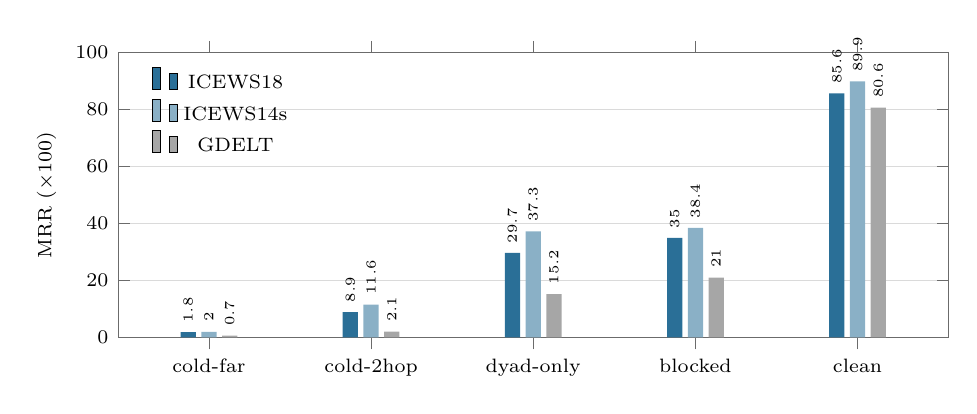
\begin{tikzpicture}
  \begin{axis}[
    ybar, width=\linewidth, height=5.2cm,
    bar width=5.5pt, ymin=0, ymax=100,
    ylabel={MRR ($\times 100$)}, ylabel style={font=\scriptsize},
    symbolic x coords={cold-far,cold-2hop,dyad-only,blocked,clean},
    xtick=data, tick label style={font=\scriptsize},
    enlarge x limits=0.14,
    legend style={at={(0.03,0.97)}, anchor=north west, legend columns=1,
                  font=\scriptsize, draw=none, fill=none},
    axis line style={cGrey}, tick style={cGrey},
    ymajorgrids, grid style={cGrey!25},
    nodes near coords, nodes near coords style={font=\tiny, /pgf/number format/fixed, /pgf/number format/precision=1, rotate=90, anchor=west},
  ]
    \addplot[fill=cDyad, draw=none] coordinates {
      (cold-far,1.84) (cold-2hop,8.93) (dyad-only,29.71) (blocked,34.99) (clean,85.64)};
    \addplot[fill=cDyad!55, draw=none] coordinates {
      (cold-far,2.01) (cold-2hop,11.57) (dyad-only,37.26) (blocked,38.43) (clean,89.93)};
    \addplot[fill=cGrey!60, draw=none] coordinates {
      (cold-far,0.65) (cold-2hop,2.05) (dyad-only,15.20) (blocked,21.03) (clean,80.64)};
    \legend{ICEWS18, ICEWS14s, GDELT}
  \end{axis}
\end{tikzpicture}

  \caption{\textbf{MRR by stratum on the three event datasets} (three seeds). The profile is the same on all three: the clean stratum is solved, the blocked and dyad-only strata are where a copy mechanism fails and where \model{} earns its margin, and the two cold strata are where the remaining headroom lies. GDELT, whose fifteen-minute snapshots make every stratum sparser, is lower everywhere but keeps the ordering.}
  \label{fig:strata-results}
\end{figure}

\Cref{fig:strata-results} repeats the stratified view on ICEWS14s and GDELT. The profile is identical across the three event datasets, which is what one expects of strata defined from the data rather than from the model: the clean stratum sits above 80 MRR everywhere, the blocked and dyad-only strata in the 15 to 40 range, and the cold strata near zero. The same figure says why GDELT is the hardest benchmark in the suite despite its small vocabulary: at fifteen-minute resolution its dyad streams are sparse, and every stratum except the clean one is a third to a half lower than on ICEWS.

\section{Conclusion}
\label{sec:conclusion}

We asked what unit of evidence a temporal knowledge graph forecaster should read, and measured the answer before modelling it. The dyad, the ordered entity pair with the typed stream of every event between its members, carries information that the query pair does not: a quarter of ICEWS queries have an answer that only the dyad can see, and a counter that reads the dyad with no training matches a published model that reads the query pair with a great deal of it. \model{} turns that measurement into a model: a superposition of intensities, with a Transformer over the dyad's event stream at its centre, a path intensity that composes a stream with a typed edge, and attention across the candidates of a query. Over three seeds it sets the best published MRR and \hone{} on YAGO and WIKI, the best \hone{} on GDELT, and exceeds every method with released code on ICEWS18 and ICEWS14s. The stratified analysis shows each intensity acting where the data said it would, and shows as plainly where the model does not act: a third of ICEWS queries whose answer never interacted with the subject remain largely out of reach, and three recent methods without released code report higher aggregate numbers on those benchmarks. Reaching the cold strata, and settling the comparison with those methods under one protocol, are the two open ends of this work. The code, the diagnostic and every result file are released so that both can be taken up.


\bibliographystyle{plain}
\bibliography{references}

\end{document}
